\documentclass[tikz,border=10pt]{standalone}
\usepackage{tikz}
\usetikzlibrary{arrows.meta,calc}

\begin{document}
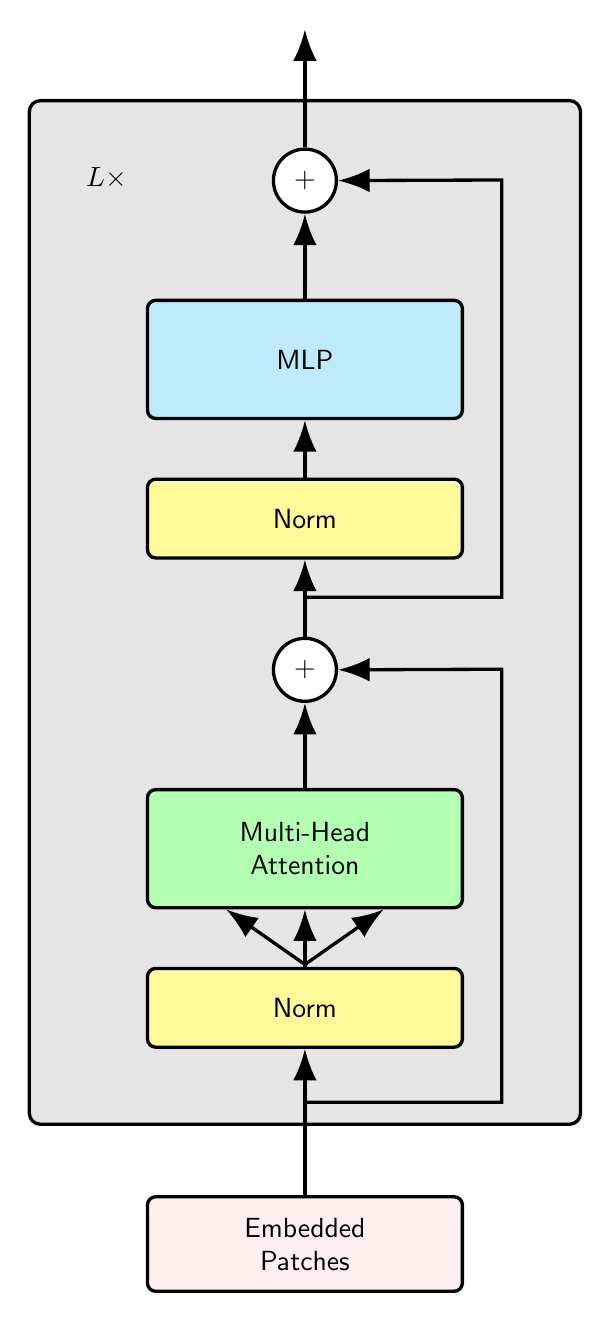
\begin{tikzpicture}[
  font=\sffamily,
  >={Latex[length=4mm,width=3mm]},
  line/.style={very thick, draw=black},
  box/.style={draw, very thick, rounded corners=3pt, align=center, minimum width=40mm},
  outer/.style={draw, very thick, rounded corners=4pt, fill=gray!20, minimum width=70mm, minimum height=130mm},
  norm/.style={box, fill=yellow!40, minimum height=10mm},
  mha/.style={box, fill=green!30, minimum height=15mm},
  mlp/.style={box, fill=cyan!25, minimum height=15mm},
  emb/.style={box, fill=pink!25, minimum height=12mm},
  add/.style={draw, very thick, circle, fill=white, minimum size=8mm, inner sep=0pt}
]

% ===== Outer container =====
\node[outer] (O) at (0,0) {};

% L x label
\node[font=\bfseries] at ($(O.north west)+(10mm,-10mm)$) {$L\times$};

% ===== Embedded patches (outside) =====
\node[emb] (E) at ($(O.south)+(0,-15mm)$) {Embedded\\Patches};

% ===== Inside blocks (bottom -> top) =====
\node[norm] (N1) at ($(O.south)+(0,15mm)$) {Norm};
\node[mha]  (A)  at ($(N1.north)+(0,15mm)$) {Multi-Head\\Attention};
\node[add]  (P1) at ($(A.north)+(0,15mm)$) {$+$};

\node[norm] (N2) at ($(P1.north)+(0,15mm)$) {Norm};
\node[mlp]  (M)  at ($(N2.north)+(0,15mm)$) {MLP};
\node[add]  (P2) at ($(M.north)+(0,15mm)$) {$+$};

% ===== Main vertical flow (until N1) =====
\draw[line,->] (E.north) -- (N1.south);

% ===== "さすまた" arrows into Multi-Head Attention =====
\coordinate (S) at ($(A.south)+(0,-7mm)$); % branch point
\draw[line,-] (N1.north) -- (S);
\draw[line,->] (S) -- ($(A.south)+(-10mm,0mm)$);
\draw[line,->] (S) -- ($(A.south)+(0mm,0mm)$);
\draw[line,->] (S) -- ($(A.south)+(10mm,0mm)$);

% ===== Continue main path =====
\draw[line,->] (A.north) -- (P1.south);
\draw[line,->] (P1.north) -- (N2.south);
\draw[line,->] (N2.north) -- (M.south);
\draw[line,->] (M.north) -- (P2.south);
\draw[line,->] (P2.north) -- ($(P2.north)+(0,15mm)$);

% ===== Residual connections (right-side) =====
\coordinate (rin1) at ($(O.south)+(0,3mm)$);
\draw[line,->] (rin1) -- ++(25mm,0mm) -- ++(0mm,55mm) -- ($(P1.east)$);
\draw[line,->] ($(P1.north)+(0,5mm)$) -- ++(25mm,0mm) -- ++(0mm,53mm) -- (P2.east);

\end{tikzpicture}
\end{document}
